%!TEX root = ../diss.tex
\tikzstyle{element}=[rectangle, thick,
                     inner sep=0.1cm, rounded corners]
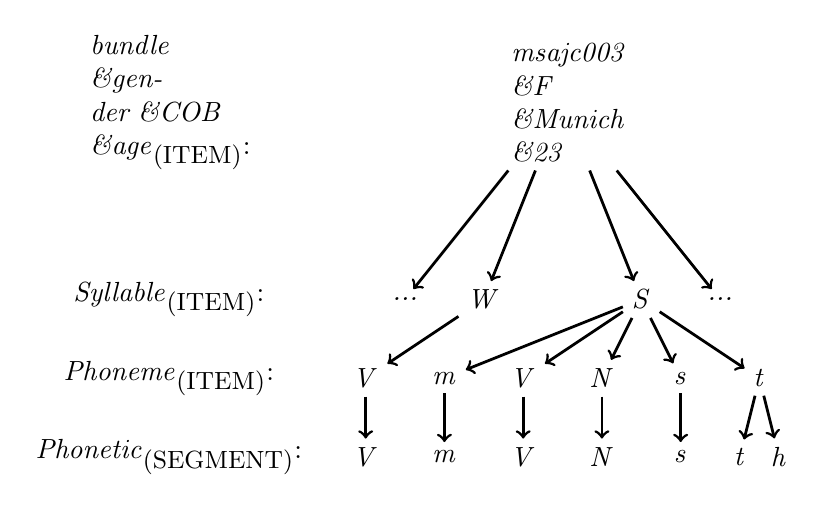
\begin{tikzpicture}

%%%%%%%%%%%%%%%%%%
%%%%%%%%%%%%%%%%%%
\node (Text) at (-5, 5.5) [element, text width = 2cm] {\textit{bundle \&gender \&COB \&age}\textsubscript{\small{(ITEM)}}:}; 

\node (amongst_Text) at (0, 5.5) [element, text width = 1.3cm] {\textit{msajc003\\ \&F \\\&Munich \\\&23}};

%%%%%%%%%%%%%%%%%%
\node (Syllable) at (-5, 3) [element] {\textit{Syllable}\textsubscript{\small{(ITEM)}}:}; 

\node (left_etc) at (-2, 3) [element] {\textit{...}};

\node (W_Syllable) at (-1, 3) [element] {\textit{W}};

\node (S_Syllable) at (1, 3) [element] {\textit{S}};

\node (right_etc) at (2, 3) [element] {\textit{...}};

%%%%%%%%%%%%%%%%%%
\node (Phoneme) at (-5, 2) [element] {\textit{Phoneme}\textsubscript{\small{(ITEM)}}:}; 

\node (V1_Phoneme) at (-2.5, 2) [element] {\textit{V}};

\node (m_Phoneme) at (-1.5, 2) [element] {\textit{m}};

\node (V2_Phoneme) at (-0.5, 2) [element] {\textit{V}};

\node (N_Phoneme) at (0.5, 2) [element] {\textit{N}};

\node (s_Phoneme) at (1.5, 2) [element] {\textit{s}};

\node (t_Phoneme) at (2.5, 2) [element] {\textit{t}};

%%%%%%%%%%%%%%%%%%%
\node (Phonetic) at (-5, 1) [element] {\textit{Phonetic}\textsubscript{\small{(SEGMENT)}}:}; 

\node (V1_Phonetic) at (-2.5, 1) [element] {\textit{V}};

\node (m_Phonetic) at (-1.5, 1) [element] {\textit{m}};

\node (V2_Phonetic) at (-0.5, 1) [element] {\textit{V}};

\node (N_Phonetic) at (0.5, 1) [element] {\textit{N}};

\node (s_Phonetic) at (1.5, 1) [element] {\textit{s}};

\node (t_Phonetic) at (2.25, 1) [element] {\textit{t}};

\node (h_Phonetic) at (2.75, 1) [element] {\textit{h}};


%%%%%%%%%%%%%%%%%%%%
%%%%%%%%%%%%%%%%%%%%
\draw [->, line width=1] (amongst_Text) to (left_etc);

\draw [->, line width=1] (amongst_Text) to (W_Syllable);

\draw [->, line width=1] (amongst_Text) to (S_Syllable);

\draw [->, line width=1] (amongst_Text) to (right_etc);

%%%%%%%%%%%%%%%%%%%%
\draw [->, line width=1] (W_Syllable) to (V1_Phoneme);

\draw [->, line width=1] (S_Syllable) to (m_Phoneme);

\draw [->, line width=1] (S_Syllable) to (V2_Phoneme);

\draw [->, line width=1] (S_Syllable) to (N_Phoneme);

\draw [->, line width=1] (S_Syllable) to (s_Phoneme);

\draw [->, line width=1] (S_Syllable) to (t_Phoneme);

%%%%%%%%%%%%%%%%%%%%
\draw [->, line width=1] (V1_Phoneme) to (V1_Phonetic);

\draw [->, line width=1] (m_Phoneme) to (m_Phonetic);

\draw [->, line width=1] (V2_Phoneme) to (V2_Phonetic);

\draw [->, line width=1] (N_Phoneme) to (N_Phonetic);

\draw [->, line width=1] (s_Phoneme) to (s_Phonetic);

\draw [->, line width=1] (t_Phoneme) to (t_Phonetic);

\draw [->, line width=1] (t_Phoneme) to (h_Phonetic);

\end{tikzpicture}
